\documentclass[ejs,preprint]{imsart}

% will be filled by editor:
\doi{10.1214/154957804100000000}
\pubyear{0000}
\volume{0}
\firstpage{0}
\lastpage{0}
%\arxiv{}

%\usepackage{color}
\usepackage{amsthm,amsmath,amssymb}
\usepackage{graphicx}
%\usepackage{graphicx}
%\usepackage{esint}

\newtheorem{definition}{Definition}
\newtheorem{proposition}{Proposition}
\newtheorem{theorem}{Theorem}

\newcommand\E{\mathbb{E}}
%\newcommand\Pr{\mathbb{P}}

\newcommand\cbayes{C^{\mathrm{Bayes}}}
\newcommand\crpnhat{\hat{C}_{n}^{\mathrm{RP}}}
\newcommand\crpnhatstar{\hat{C}_{n}^{\mathrm{RP*}}}
\newcommand\risk{\mathcal{L}}
\newcommand\rrisk{\mathcal{R}}
\newcommand\cabayes{C^{A-\mathrm{Bayes}}}
\newcommand\rabayes{\rrisk^{A-\mathrm{Bayes}}}

\begin{document}

\begin{frontmatter}

% "Title of the Paper"
\title{Axis-Aligned RPE Classification \& Bayesian Random Projection Optimization}
\runtitle{Axis-Aligned RPE \& Bayesian RP Optimization}

% indicate corresponding author with \corref{}
% \author{\fnms{John} \snm{Smith}\thanksref{t2}\corref{}\ead[label=e1]{smith@foo.com}\ead[label=e2,url]{www.foo.com}}
% \thankstext{t2}{Thanks to somebody} 
% \address{line 1\\ line 2\\ \printead{e1}\\ \printead{e2}}

\author{\fnms{Benjamin J.} \snm{Li}\thanksref{t1}\ead[label=e1]{jiachengli@college.harvard.edu}}
\address{Department of Mathematics\\
Harvard University\\
\printead{e1}}
\and
\author{\fnms{Timothy I.} \snm{Cannings}\ead[label=e2]{t.cannings@statlab.cam.ac.uk}}
\address{Statistical Laboratory\\
University of Cambridge\\
\printead{e2}}

\thankstext{t1}{Thanks to my summer research advisor Richard J. Samworth at the Statistical Laboratory, University of Cambridge, under whom this research was performed.} 

\runauthor{B. J. Li and T. I. Cannings}

%\begin{abstract}
%\end{abstract}

%\begin{keyword}[class=MSC]
%\kwd[Primary ]{}
%\kwd{}
%\kwd[; secondary ]{}
%\end{keyword}

%\begin{keyword}
%\kwd{}
%\kwd{}
%\end{keyword}

% history:
% \received{\smonth{1} \syear{0000}}

%\tableofcontents

\end{frontmatter}











\section{Background}

\subsection{Motivation}

A supervised classification problem requires prediction of class labels $Y$ from covariates $X$ given training data. Increasingly often, classification problems are high-dimensional: specifically, the dimension of the feature vectors $p$ is greater than the length of the training set $n$. This violates assumptions in many classification methods, causing poor performance or failure (as in linear discriminant analysis, where the sample covariance matrix when $p\geq n$ is not invertible). Current methods tailored to this situation make strong linearity, sparsity, and/or independence assumptions, as surveyed in \cite{CS15}.

This limits their expressivity, in exchange for statistical power on problems that do fit the assumptions. Ensembling, as used for instance in random forests \cite{Breiman01}, is able to expand expressivity. Random forest performs bootstrap aggregation (bagging), in which the votes of component classifiers trained on bootstrapped data are aggregated, which enables, for instance, nonlinear decision boundaries with linear base classifiers.

But bagging is unhelpful in high-dimensional classification -- instead of training component classifiers on ``row-sampled'' data (which effectively reduces $n$, not $p$!), it would be nice to train them on ``column-sampled'' data. This motivation is especially strong because we have a powerful guarantee on this ``column-sampling.''

The Johnson-Lindenstrauss Lemma \cite{DG03} states that for any $\epsilon\in(0,1)$ there is some projection $A$ to $\mathbb R^d$ where $d>\frac{8\log n}{\epsilon^2}$ \footnote{Note that this is independent of $p$.} that preserves squared pairwise distances between data points within $\epsilon$, and in fact this matrix can be found stochastically in polynomial time.


\subsection{Introduction}

Random projection ensemble (RPE) classification is a very recent method developed to solve the problem of high-dimensional classification.
The fundamental idea is that we can improve the expressiveness and power of any base classifier $\hat C$ under a sufficient dimensionality reduction assumption by applying $\hat C$ to lower-dimensional projections of the feature vectors $A_i X$ and aggregating their responses.

The specifics of the methodology discussed in \cite{CS15} involve drawing $B_{1}\times B_{2}$ $d$-dimensional projections from Haar measure on the space of all such projection matrices, running the base classifier with each of these projections, and then choosing the best of every $B_{2}$ projections, giving a final ensemble of $B_{1}$ projections.

In this paper, we detail two separate improvements, corresponding exactly to the two separate halves of the bound on excess test risk in \cite{CS15}. (Below we use notation which we will go over in Sections~\ref{sec:glossary} and \ref{sec:review}).

\subsubsection{First half}

In the first half (Theorem 1), no distribution on the $B_1$ matrices $\{A_i\}$ is assumed, and it is shown that
\begin{equation}
\risk(\crpnhat) - \risk(\crpnhatstar) \leq O\left(\frac{1}{B_1}\right)
\label{eqn:first-half}
\end{equation}
asymptotically in $B_1$.

As the dimension $p$ of the original data goes up, the space of projections $\mathbb{R}^p\to\mathbb{R}^d$ grows exponentially, as the paper remarks.
It makes sense to restrict the set of projections on $A$ to be axis-aligned. An axis-aligned projection simply picks $d$ basis vectors and drops the rest, bounding the set to $\binom{p}{d}\leq p^{d}/d!$ which is polynomial in $d$.

It turns out that restricting projections to the axis-aligned subspace causes the bound in Equation~\ref{eqn:first-half} to become exponential in $B_1$, and for the bound to hold non-asymptotically under certain conditions!

\subsubsection{Second half}

In the second half (Theorem 2, Proposition 3, and Theorem 5), the best-of-$B_2$ algorithm (hereafter referred to as \textit{bruteforce}) is assumed and it is shown that with $A_i$ chosen by this algorithm, 
\begin{align*}
\risk(\crpnhatstar) - \rrisk(\cbayes)
	&\leq \frac1{\alpha(1-\alpha)}\big[
			\E(\risk_n^{A_1})-\rrisk(\cbayes)
		\big] \qquad\text{(Theorem 2)} \\
	&\leq \frac1{\alpha(1-\alpha)}\big[
			\hat{L}_n^* - \rrisk(\cbayes) + \epsilon_n \\
	&\quad	+ \text{terms from Assumption (A.2)}
		\big] \qquad\text{(Proposition 3)} \\
	&\leq \frac1{\alpha(1-\alpha)}\big[
			(\risk_n^{A^*} - \rrisk^{A^*-\mathrm{Bayes}}) \\
	&\quad	+ (\epsilon_n - \epsilon_n^{A^*}) \\
	&\quad	+ \text{terms from Assumption (A.2)}
		\big] \qquad\text{(Theorem 5)}
\end{align*}
The sum of this with the first-half inequality is then the desired bound.

Choosing the $A_i$ by brute force reuses no previous information. In addition, unlike the tidy first-half inequality, the second-half inequality requires the unnatural Assumption (A.2) and multiple steps to prove, resulting in a bound with complicated terms.

A more elegant way to derive good projection matrices would be to sample them from the posterior distribution of $A^*$, the true sufficient dimension reduction matrix from Assumption (A.3). We give a Metropolis-Hastings algorithm for this, and prove a new second-half bound.

\subsection{Glossary}\label{sec:glossary}
\begin{definition}
The \textbf{risk} of a classifier is defined as the \textbf{misclassification
rate} 
\[
\rrisk(C):=\mathbb{P}\left\{ C(X)\neq Y\right\} 
\]
When $C$ is based on data, we write $\hat{C}$ and use the letter
$\risk$ instead of $\rrisk$ to denote risk. The \textbf{excess risk}
of $\hat{C}$ is defined by $\risk(\hat{C})-\rrisk(C^{\mathrm{Bayes}})$.
\end{definition}
There are analogous definitions for estimates of risk based on the
training data:
\begin{definition}
The \textbf{test risk} of a classifier (which I will sometimes refer
to as the \textbf{risk estimate}) replaces $\risk$ with some estimator
of risk based on the data $\hat{L}$, and the \textbf{excess test
risk} (or \textbf{excess risk estimate}) is similarly $\hat{L}(\hat{\theta})-\rrisk(\hat{\theta}^{\mathrm{Bayes}})$.
\end{definition}
Finally, central to the first-half bound, we define the projection matrix space,
and the distribution on it:
\begin{definition}
$\mathcal{A}$ is the subset of $d$-projection matrices that we draw
our random projections from. A random matrix $A$ is a matrix-valued
random variable with some distribution on $\mathcal{A}$.
\end{definition}

There are also some abbreviations we will use throughout the paper:
\begin{itemize}
\item RPE - random projection ensemble (classification)
\item RPE-H - RPE with matrices drawn from Haar measure
\item RPE-A - RPE with uniformly drawn axis-aligned matrices
\end{itemize}

\subsection{Review of RPE theory}\label{sec:review}

The original method made three assumptions in order to deduce that
excess risk $\risk(\crpnhat)-\rrisk(\cbayes)$ is bounded by a sum
of expressions that do not depend on $p$. They are, in order and
paraphrased:\\


\noindent \textbf{Assumption (A.1).} $G_{n,1}$ and $G_{n,2}$ have
second derivatives at the voting threshold $\alpha$, where, given
the true joint distribution of the training data $(X,Y)$, $G_{n,i}$
is the CDF of the probability that the base classifier $\hat{C}_{n}$
will classify a random projection of $X$ as class $i$.\\


This assumption is used to show that the risk of the finite
RPE classifier $\crpnhat$ (with choices of base classifier $\hat{C}_{n}$,
voting threshold $\alpha$, and finite ensemble size parameters $B_{1}$
and $B_{2}$) is well-approximated by that of the infinite-simulation
RPE classifier $\crpnhatstar$ (with the same choices of $\hat{C}_{n}$
and $\alpha$). This result is \textbf{Theorem 1}, and does not involve
the distribution on the projection matrices $A_{i}$ other than that
they are independent and identically distributed, and independent
of $(X,Y)$. This concludes the first-half bound.


\textbf{Theorem 2}, bounding $\risk(\crpnhatstar)-\rrisk(\cbayes)$,
does not involve the distribution on the projection matrices $A_{i}$
other than that they are independent and identically distributed,
and independent of $(X,Y)$. Thus, this result pulls smoothly into
the axis-aligned case.


The next assumption involves the production of a good selection of
random projections by taking the best projection in each row from
a $B_{1}\times B_{2}$-sized grid of i.i.d. random projections from
some base distribution (Haar measure as generally discussed in the
original paper). To make conclusions about the test error of such
a screened-Haar RPE classifier, we define $\beta_{n}(j)$ as the discrete
CDF of $n\left(\hat{L}_{n}^{A}-\hat{L}_{n}^{*}\right)$ (which is
the random variable $n\hat{L}_{n}^{A}=\sum_{(x,y)}I(\hat{C}_{n}^{A}(x)\neq y)$
minus a constant, where $X,Y$ are known and $A$ is random).\\


\noindent \textbf{Assumption (A.2).} There is some $B_{0}\in(0,1)$
and $\beta,\rho>0$ such that the histogram $\beta_{n}(j)$ is bounded
below by the discrete CDF $\beta_{0}+\frac{\beta j^{\rho}}{n^{\rho}}$
for all $j$ below $n\left(\frac{\log^{2}B_{2}}{\beta B_{2}}\right)^{1/\rho}+1$.
It is particularly noted that as $B_{2}$ goes up, the strength of
the condition decreases (a smaller bit of the left side of the CDF
is constrained).\\


From this, \textbf{Proposition 3} bounds the expected excess risk
$\mathbb{E}(\risk_{n}^{A_{1}})-\rrisk(\cbayes)$ of a $B_{2}$-filtered
projection by an expression involving $\hat{L}_{n}^{*}-\rrisk(\cbayes)$,
the minimum excess risk estimate over all $A\in\mathcal A$,
which leads naturally to the next step of trying to bound that. Intuitively,
we expect this to be small when the Bayes classifier indeed only takes
into account $d$ of the dimensions, which leads to the following
definition and assumption:

\begin{definition}
Let $\cabayes$ be the \textbf{projected Bayes classifier}, defined
as the Bayes classifier on the joint distribution $(AX,Y)$, and $\rabayes$
its risk.
\end{definition}


\noindent \textbf{Assumption (A.3).} There is some projection $A^{*}\in\mathcal{A}$
such that the Bayes classifier and the projected Bayes classifier
are the same except on a set of measure zero.\\


\textbf{Proposition 4} goes to show that (A.3) holds under the sufficient
dimension reduction condition (there exists a dimension reduction
$R$ such that $R(X)$ is sufficient, ie. $Y\,|\,R(X)$ has the same
distribution as $Y\,|\,X$). Naturally one would expect that if (A.3)
holds, $\hat{L}_{n}^{*}$ would be close to $\rrisk(\cbayes)$, which
is quantified in \textbf{Theorem 5}.





















\section{Axis-aligned RPE theory}

\subsection{$G_{n,i}$ curves}

\begin{figure}
\begin{centering}
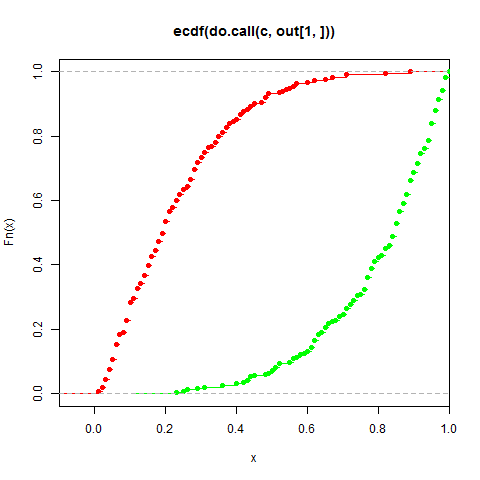
\includegraphics[scale=0.35]{G_ni}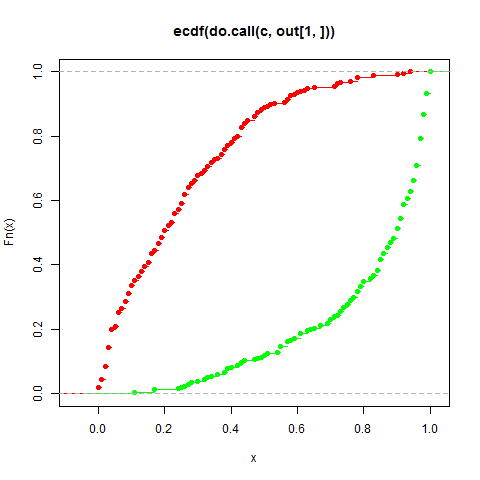
\includegraphics[scale=0.35]{G_ni_axis}
\par\end{centering}

\caption{The empirical $G_{n,i}$ curves for the standard run ($B_{1}=B_{2}=100$)
of Model 1 ($n_{\mathrm{train}}=50$) with RPE-H LDA (left) versus
RPE-A LDA (right), averaged over 10 instances.}

\label{fig:std-run-g-curves}
\end{figure}


The natural place to wedge in an axis-aligned version of the method
would be right in the beginning at Assumption (A.1). Central to
Theorem 1, the most involved theoretical result in the paper, are
the $G_{n,i}$ curves. They are estimated and plotted in Figure~\ref{fig:std-run-g-curves}
for a standard run of Model 1 with both RPE-H LDA and RPE-A LDA. (Note
that adjusting $n_{\mathrm{train}}$ changes the shape of these curves,
which is why they've been averaged over 10 instances instead of simply
run on 10 times more data.)

Although it's not evident in these plots, observe that finite $\mathcal{A}$
implies a discrete distribution on $A$, which implies that the $G_{n,i}$
are step functions -- a much stronger assumption than second-differentiability
at the voting threshold $\alpha$!

\begin{figure}
\begin{centering}
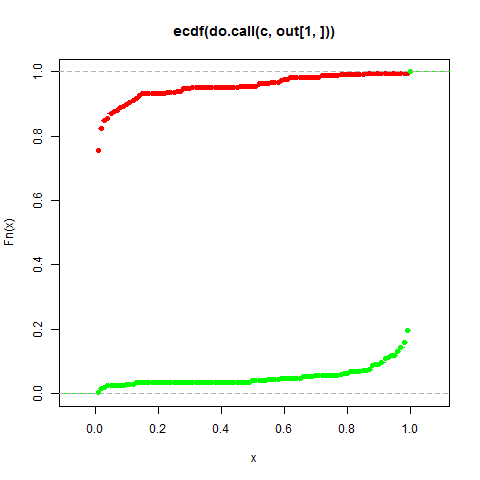
\includegraphics[scale=0.35]{G_ni_mini}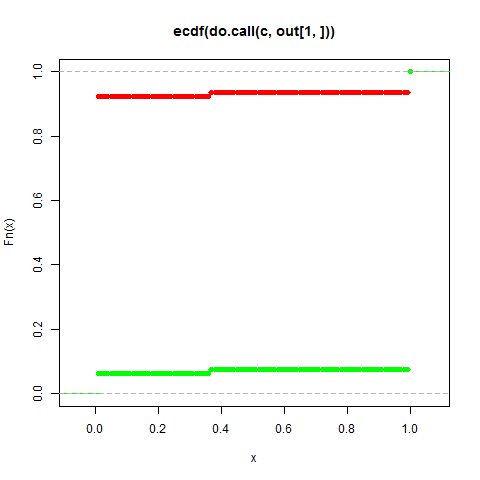
\includegraphics[scale=0.35]{G_ni_mini_axis}
\par\end{centering}

\caption{The empirical $G_{n,i}$ curves for $p=5$
and $d=2$, again with RPE-H LDA (left) and RPE-A LDA (right), averaged
over 10 instances. The difference is much clearer.}


\label{fig:mini-run-g-curves}
\end{figure}


As a much clearer illustration, Figure~\ref{fig:mini-run-g-curves} shows
these curves with $p=5$ and $d=2$.

\subsection{Effect of axis-alignment on second-half bound}

Restricting $\mathcal A$ to axis-aligned projections does not affect Theorem 2, which is independent of the distribution of $A$.

The CDF $\beta_{n}(j)$ can still be defined, where $A$ is now distributed
uniformly on the set of axis-aligned projection matrices, so Assumption
(A.2) and Proposition 3 can remain unchanged (where $A_{1}$ is now
distributed as $B_{2}$-filtered axis-aligned projection matrices).

Assumption (A.3) has a simple modification (compatible with Proposition
4) to make Theorem 5 hold for axis-aligned projections:\\


\noindent \textbf{Assumption (A.3').} There is some \emph{axis-aligned}
projection $A^{*}\in\mathcal{A}$ such that the Bayes classifier and
the projected Bayes classifier are the same except on a set of measure
zero.\\


Thus, all that's left to fill in are the new (A.1) and Theorem 1 (and
replacing the Theorem 1-derived part in Theorem 5's bound with the
corresponding new and improved expression).


\subsection{New theorem}

We revise Assumption (A.1):\\

\noindent \textbf{Assumption (A.1$'$).} $G_{n,1}$ and $G_{n,2}$ are
constant in a neighborhood of $\alpha$.\\

It is easy to show that this assumption holds for our axis-aligned
case.

\begin{proposition}
Allowing infinitesimal perturbation of $\alpha$\footnote{Practically, we would choose $\alpha$ with its distance to an element of $R$ in mind, as we discuss later, so this is somewhat irrelevant.}, Assumption (A.1$'$) holds for $\mathcal{A}$ as the set of axis-aligned
$d\times p$ projections (or any subset thereof) and $A$ a matrix-valued
random variable with this set as its support, with some distribution\footnote{For example, uniform over $\mathcal{A}$, or as is done in the package,
chosen from the best of $B_{2}$ uniform candidates.} given by probabilities $q_{B}$ for all $B\in\mathcal{A}$.
\end{proposition}


\begin{proof}
We have that 
\begin{eqnarray*}
G_{n,1}(\alpha) & = & \mathbb{P}\left\{ \mathbb{P}\left\{ \hat{C}_{n}^{A}(X)=1\,\Big|\,X\right\} \leq\alpha\,\Big|\,Y=1\right\} \\
 & = & \mathbb{P}\left\{ \sum_{B\in\mathcal{A}}q_{B}I\left\{ \hat{C}_{n}^{B}(X)=1\right\} \leq\alpha\,\Big|\,Y=1\right\} 
\end{eqnarray*}
 is the CDF of a finite weighted sum of indicators. It can be seen
as a step function with up to $||\mathcal{A}||$ jumps; let the set of the
horizontal locations of these jumps be $R_{1}$ and let the corresponding
vertical heights be $s_{r}$ (ie. such that $\sum_{r\in R_{1}}s_{r}=1$).
Note that $R_{1}$ has Lebesgue measure zero inside $[0,1]$ and $G_{n,1}$
is flat (thus has zero first and second derivatives) outside of $R_{1}$.

The same holds for $G_{n,2}$; let the horizontal locations of its
jumps be $R_{2}$ and the vertical heights be $t_{r}$ analogously.

Then outside of the set $R=R_{1}\cup R_{2}$, $G_{n,1}$ and $G_{n,2}$ are locally constant. If we allow infinitesimal perturbation of $\alpha$, it will never fall into this set.
\end{proof}


Note that the set $R$ has cardinality at most $2||\mathcal{A}||=2\binom{p}{d}\leq2\frac{p^{d}}{d!}$.\\


Now we design an analogous version of Theorem 1:\\


\noindent \textbf{Theorem 1$'$.} \emph{Assume (A.1$'$). Then 
\[
\risk\left(\crpnhat\right)-\risk\left(\crpnhatstar\right)=o\left(B_{1}^{-M}\right)
\]
 as $B_{1}\to\infty$ for all $M\in\mathbb{N}$.}\footnote{\noindent Note that here $\crpnhatstar$ represents the infinite axis-aligned
projection RPE classifier, so that although this bound is tighter,
the infinite projection classifier we're approximating may be farther
from the Bayes classifier than the general case. But this doesn't affect our theory, as
we modified (A.3) so that $A^{*}$ must be axis-aligned.}

Moreover, there exists some $C>0$ such that for all $B_1\geq C$, the non-asymptotic bound
\[
\risk\left(\crpnhat\right)-\risk\left(\crpnhatstar\right)=e^{-2\log^2 B_1}
\]
holds.


\begin{proof}
As before we have 
\begin{eqnarray*}
\risk(\crpnhat) & = & \pi_{1}\mathbb{P}\left\{ \crpnhat(X)=2\,|\,Y=1\right\} +\pi_{2}\mathbb{P}\left\{ \crpnhat(X)=1\,|\,Y=2\right\} \\
 & = & \pi_{1}\mathbb{P}\left\{ \hat{\nu}_{n}^{B_{1}}(X)<\alpha\,|\,Y=1\right\} +\pi_{2}\mathbb{P}\left\{ \hat{\nu}_{n}^{B_{1}}(X)\geq\alpha\,|\,Y=2\right\} 
\end{eqnarray*}
 where $\hat{\nu}_{n}^{B_{1}}(x):=\frac{1}{B_{1}}\sum_{b_{1}=1}^{B_{1}}I\left\{ \hat{C}_{n}^{A_{b_{1}}}(x)=1\right\} $.
Conditional on the mean $\hat{\mu}_{n}(X)=\theta$ of the $I\left\{ \hat{C}_{n}^{A_{b_{1}}}(x)=1\right\} $,
they are i.i.d. $\mathrm{Bern}(\theta)$. As $G_{n,1}$ is the CDF
of $\hat{\mu}_{n}(X)\,|\,\{Y=1\}$, we can write 
\begin{eqnarray*}
\mathbb{P}\left\{ \hat{\nu}_{n}^{B_{1}}(X)<\alpha\,|\,Y=1\right\}  & = & \int_{0}^{1}\!\mathbb{P}\left\{ \frac{1}{B_{1}}\sum_{b_{1}=1}^{B_{1}}I\left\{ \hat{C}_{n}^{A_{b_{1}}}(x)=1\right\} <\alpha\,\bigg|\,\hat{\mu}_{n}(X)=\theta\right\} \,dG_{n,1}(\theta)\\
 & = & \int_{0}^{1}\!\mathbb{P}(T<B_{1}\alpha)\,dG_{n,1}(\theta)
\end{eqnarray*}
 for $T\sim\mathrm{Bin}(B_{1},\theta)$. Combining with the similar
result for $G_{n,2}$ gives 
\[
\risk(\crpnhat)=\pi_{2}+\int_{0}^{1}\!\mathbb{P}(T<B_{1}\alpha)\,dG_{n}^{\circ}(\theta)
\]
 where $G_{n}^{\circ}=\pi_{1}G_{n,1}-\pi_{2}G_{n,2}$. Subtracting the statement 
\[
\risk\left(\crpnhatstar\right)=\pi_{1}G_{n,1}(\alpha)+\pi_{2}\left(1-G_{n,2}(\alpha)\right)
\]
 gives 
\[
\risk\left(\crpnhat\right)-\risk\left(\crpnhatstar\right)=\int_{0}^{1}\!\mathbb{P}(T<B_{1}\alpha)-I\{\theta<\alpha\}\,dG_{n}^{\circ}(\theta)
\]


As before we show that 
\[
\int_{0}^{1}\!\mathbb{P}(T<B_{1}\alpha)-I\{\theta<\alpha\}\,dG_{n}^{\circ}(\theta)=\int_{\alpha-\epsilon}^{\alpha+\epsilon}\!\mathbb{P}(T<B_{1}\alpha)-I\{\theta<\alpha\}\,dG_{n}^{\circ}(\theta)+o(B_{1}^{-M})
\]
 as $B_{1}\to\infty$ for all $M\in\mathbb{N}$, by Hoeffding's inequality:
for $\epsilon=\frac{\log B_{1}}{\sqrt{B_{1}}}$ and all $M$ we have
\[
\sup_{|\theta-\alpha|\geq\epsilon}\left|\mathbb{P}(T<B_{1}\alpha)-I\{\theta<\alpha\}\right|\leq\sup_{|\theta-\alpha|\geq\epsilon}\exp\left\{ -2B_{1}(\theta-\alpha)^{2}\right\} \leq e^{-2\log^{2}B_{1}}=o(B_{1}^{-M})
\]


Let $I=(\alpha-\epsilon,\alpha+\epsilon)$. Note that $G_{n,1}$ is
the CDF of a discrete random variable with values $r\in R_{1}$ and
probabilities $s_{r}$, so that 
\begin{eqnarray*}
\int_{\alpha-\epsilon}^{\alpha+\epsilon}\!\mathbb{P}(T<B_{1}\alpha)-I\{\theta<\alpha\}\,dG_{n}^{\circ}(\theta) & = & \pi_{1}\sum_{r\in R_{1}\cap I}s_{r}\left(\mathbb{P}(T<B_{1}\alpha)-I\{r<\alpha\}\right)\\
 &  & -\pi_{2}\sum_{r\in R_{2}\cap I}s_{r}\left(\mathbb{P}(T<B_{1}\alpha)-I\{r<\alpha\}\right)
\end{eqnarray*}


From here, we can already conclude: we can make both $R_{1}\cap I$
and $R_{2}\cap I$ empty by setting $B_{1}$ high enough that $\epsilon<\min_{r\in R_{1}\cup R_{2}}|\alpha-r|$.
\end{proof}

In other words, one can get bounds exponentially close to $\crpnhatstar$
(the infinite axis-aligned projection classifier), as opposed to only
linearly close to the general infinite projection classifier.

As $\epsilon=\frac{\log B_{1}}{\sqrt{B_{1}}}$ is strictly decreasing in $B_{1}$ for all $B_{1}>1$, and has inverse $B_{1}=\exp\left(-2W_{-1}(-\frac{\epsilon}{2})\right)$ involving the Lambert $W$ function \cite{CGHJK96}, this exponential behavior kicks in non-asymptotically at
\[
B_{1}>\exp\left(-2W_{-1}\left(-\frac{\min|\alpha-r|}{2}\right)\right)
\]
which unfortunately grows very quickly in $p$ and $d$.

\subsection{Estimating $\min|\alpha-r|$}

In the process of determining this lower bound, an issue arises with the determination of $\min|\alpha-r|$.
We only know $\hat{\pi}_{1}n_{\mathrm{train}}$ elements of $R_{1}$, which is generally not anywhere close to the cardinality of $R_{1}$ (which can be as big as $2^{||\mathcal{A}||}=2^{\binom{p}{d}}$).
However, we can estimate $\min|\alpha-r_{1}|$ by the following procedure:
\begin{enumerate}
\item Smooth $\hat{g}_{n,1}$ (by, for instance, taking $\tilde{g}_{n,1}$
as the sum of Gaussians at each known element of $R_{1}$ with some
specified bandwidth).
\item Evaluate this smoothed empirical density at $\alpha$.
\item Note that on average, a $\tilde{g}_{n,1}(\alpha)\times\delta$ slice
of the density will contain $\tilde{g}_{n,1}\delta||R_{1}||$ points;
setting this to 1 gives $\delta=\frac{1}{\tilde{g}_{n,1}(\alpha)\cdot||R_{1}||}$
as our estimate for $\min|\alpha-r_{1}|$.
\end{enumerate}
Combined with previous observations, this means that generally we
need 
\[
B_{1}>\exp\left\{ -2W_{-1}\left(-\frac{1}{2^{\binom{p}{d}+1}\cdot\max_i\tilde{g}_{n,i}(\alpha)}\right)\right\} 
\]
 (where $W_{-1}$, also known as the product logarithm, vanishes
more slowly than the logarithm -- see the next section).

If $\max_i\tilde{g}_{n,i}(\alpha)$ doesn't vanish quickly enough, this
expression will be dominated by the exponential behavior of $||R||$.


\subsection{Discussion \& future work}

\begin{figure}
\begin{centering}
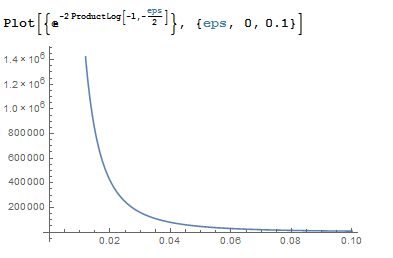
\includegraphics[scale=0.8]{aa-b1-as-func-of-eps.PNG}
\par\end{centering}

\caption{Lower bound for $B_{1}$ as a function of upper bound for $\epsilon$.}

\label{fig:b1-as-func-of-eps}
\end{figure}


Although the theorem is impressive at first glance, the lower bound
for $B_{1}$ before the exponential decay of error in Theorem 1$'$ kicks
in is very large and grows extremely quickly in $p$ and $d$, as
a result of the exponential (see Figure~\ref{fig:b1-as-func-of-eps}).
For instance, we need $\max_i g_{n,i}(\alpha)$
at a value of $2^{-\binom{p}{d}+1}$ to put the minimum $B_{1}$ for
exponential behavior at $74.2$.

This theoretical result would go hand-in-hand with a good algorithm
for choosing projections.
If we have a good method of optimizing projections, then $g_{n,1}$
and $g_{n,2}$ (the distribution functions from which we draw $r_{1}\in R_{1}$
and $r_{2}\in R_{2}$ respectively) would tend to be skewed far left
and far right respectively. Optimal values of $\alpha$ would then
be in the middle, where $R_{1}\cup R_{2}$ is much less dense, and
thus $\min|r-\alpha|$ larger, allowing for exponential behavior with
lower $B_{1}$.

\begin{figure}
\begin{centering}
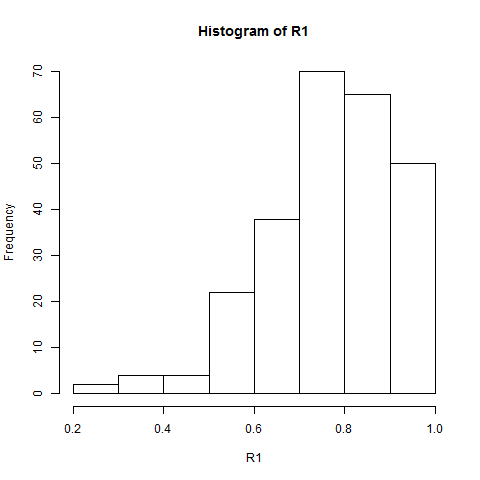
\includegraphics[scale=0.5]{r1_dist}
\par\end{centering}

\caption{$g_{n,1}$ (the distribution of $r_{1}=\mathbb{P}\left(\hat{C}_{n}^{A}(X)=1\,|\,X,Y=1\right)$)
for Model 1 with standard parameters, estimated from 10 runs.}


\label{fig:r1-dist}
\end{figure}

Even more ideally we would have an algorithm for $A_{1}$ that almost never lets $r_{1}$ or $r_{2}\in(\alpha-\epsilon,\alpha+\epsilon)$
-- then $\risk\left(\crpnhat\right)-\risk\left(\crpnhatstar\right)$ would decay exponentially in $B_{1}$ with no minimum bound on $B_{1}$! This would apply even to Haar or other base distributions on projection matrix space.

A simple example would be to have the sampler purposefully reject any such draw of $A_1$ for which $\hat r_i = \frac1n\sum_{j=1}^n I(\hat C_n^{A_1}(X)=1 \,|\, X,Y=i) \in (\alpha+\epsilon, \alpha-\epsilon)$ -- the interval can be widened to compensate for the inaccuracy of $\hat r_i$.


































\section{Bayesian random projection optimization}

The second part of this paper deals with the second-half inequality, bounding $\risk(\crpnhatstar) - \rrisk(\cbayes)$ by more efficiently sampling $B_1$ projections that comprise the ensemble.

\begin{figure}
\begin{centering}
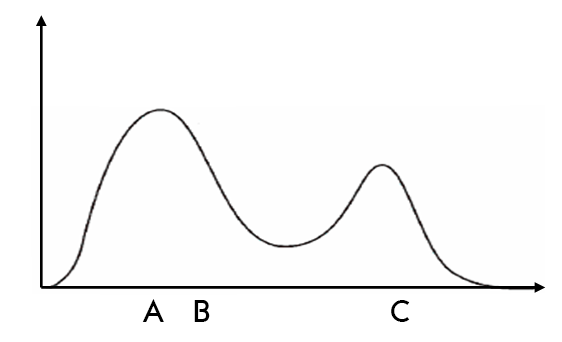
\includegraphics[scale=0.4]{illustration1}
\caption{An example posterior density $\pi(A=A^*\,|\,\mathrm{data})$, visualized in one dimension.
\label{fig:illust1}}
\par\end{centering}
\end{figure}

In Figure~\ref{fig:illust1}, point (A) would be the single (point) estimate $\widehat{A^*}$ in the original method of drawing the $A_i$; as projection with the minimum test error (``likelihood'') out of $B_2$ projections drawn from the prior (uniformly).

However, maybe the real $A^*$ is at point (B). Or possibly in an entirely separate probability cluster, at point (C). If we do greedy bruteforce optimization, we'll never get representatives from the smaller peak.

\begin{figure}
\begin{centering}
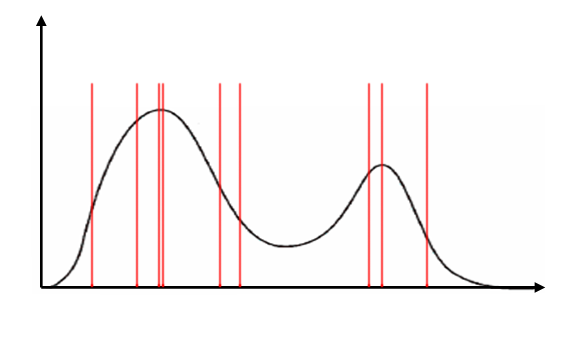
\includegraphics[scale=0.4]{illustration2}
\par\end{centering}
\caption{An ensemble representing (approximating) $\pi(A=A^*\,|\,\mathrm{data})$.}
\label{fig:illust2}
\end{figure}

The original method is basically trying to find the MAP estimate. It would be nice to use the full information of the posterior distribution, rather than just the single-point MAP estimate. The best way to do this would be to draw $B_1$ samples from $\pi$, as shown in Figure~\ref{fig:illust2}.

Here, we work directly from the sufficient dimension reduction theorem (skipping Proposition 4 and Assumption (A.3)), which we call the new \textbf{Assumption (A.3)$'$}.

\subsection{Outline}

Let $g(\pi)=\E_{A\sim\pi}(\risk_n^A)$ be our target functional. Let $\pi_0(\theta)=\delta_{A^*}(\theta)$ be the true density of $A^*$, ie.
\[
\int_R\!\pi_0(A)\,\mu(A)=I(A^*\in R\,|\,\text{true }A^*)
\]
We want to sample the $A_i$ from some $\tilde \pi_{B_2}$ such that $g(\tilde \pi_{B_2})$ is as close as possible to $g(\pi_0)=\risk_n^{A^*}$ (ie. picking up from Theorem 2).

This process is split into three steps:
\[
\tilde\pi_{B_2} \to \pi_{B_2} \to \pi \to \pi_0
\]
We start with the first arrow.

\subsection{Posterior distribution of $A^*$}

Recall the sufficient dimension reduction theorem posited the existence of a projection $A^*$ such that conditioned on $A^*X$, $X$ is independent of $Y$. Let $A^*=\theta$ be the unknown parameter in a Bayesian inference setting. Define the following quantities:

\begin{center}
\begin{tabular}{r|l}
Parameter & $\theta=A^*$ \\
Data & $D=(X,Y)$ \\
Model (likelihood) & $f(D\,|\,\theta)$ \\
Prior & $\pi(\theta)=$ Haar measure on $\mathcal{A}$ \\
Marginal & $m(D) = \int\!f(D\,|\,\theta)\pi(\theta)\,d\theta$ \\
Posterior & $\pi(\theta\,|\,D) = \frac{f(D\,|\,\theta)\pi(\theta)}{m(D)}$
\end{tabular}
\end{center}

We would like the posterior $\pi(\theta\,|\,D)$ to converge to $\delta_{A^*}$ as $n\to\infty$, which it will if we use the correct model $f$.

Note that formally we need a lot of information (including a distribution on the conditionally independent ``noise'' component $\theta^\perp(X)=(I_{p\times p}-\theta)(X)$):
\begin{equation}
f(D\,|\,\theta)=f(\theta X, \theta^\perp X,Y\,|\,\theta)=f(\theta^\perp X\,|\,\theta X, \theta)f(\theta X, Y\,|\,\theta)
\label{eqn:likelihood-decomposition}
\end{equation}
by Assumption (A.3)$'$. Clearly there is no way we can use the actual $f$ for general classification, because it would require making too many model assumptions.

\newcommand{\approxpropto}{\mathrel{\vcenter{
  \offinterlineskip\halign{\hfil$##$\cr
    \propto\cr\noalign{\kern2pt}\sim\cr\noalign{\kern-2pt}}}}}

Luckily, however, we only need a function proportional to $f(D\,|\,\theta)$ for the sampling algorithm we are about to use, and in addition, we will make some approximations. For the second term of Equation~\ref{eqn:likelihood-decomposition}, we can substitute the test accuracy of our base classifier $\hat C$:\footnote{In fact, if we are learning the $A_i$ iteratively in parallel, we could use the previous iteration's $\hat C^{\mathrm{RP}}$ for an even better approximation.}
\[
f(\theta X, Y\,|\,\theta) \approxpropto 1-\hat L_n^{\theta} = \sum_i \frac1n I (\hat C(\theta X_i) = Y_i)
\]

For the first term of Equation~\ref{eqn:likelihood-decomposition}, instead of making a model assumption about noise, we can substitute a term that represents the independence of $\theta^\perp X$ from $Y$ (requiring the estimation of conditional covariances\footnote{For example see \cite{FY98} for a method to estimate conditional covariance. Alternatively, we can approximate the conditional covariances by nonconditional covariances, which are then extremely easy to calculate.}):
\[
f(\theta^\perp X\,|\,\theta X, \theta) \approxpropto 1 - \frac{1}{p-d} \sum_i \sqrt\frac{\sigma^2_{(\theta^\perp X)_i,Y\,|\,\theta X}}{\sigma_{(\theta^\perp X)_i\,|\,\theta X}\sigma_{Y\,|\,\theta X}}
\]
However, for the rest of this paper we will focus on the accuracy term, and omit the noise independence term, which will be left to future work.

Also, to state the obvious: when faced with a classification problem for which there \emph{is} a good model for $(\theta X,Y)$ or $\theta^\perp X$ or both, plugging them in above will increase power.

\subsection{Assuming $\tilde f$ is a good approximation of $f$}

Let $\tilde f(D\,|\,\theta)$ represent one of the above approximations, and $\tilde\pi(\theta\,|\,D)$ represent the corresponding posterior derived from $\tilde f$. Next, let $\tilde \pi_{B_2}$ and $\pi_{B_2}$ represent the distribution of a sample from a Markov chain with corresponding stationary distribution after $B_2$ iterations (more on this later). The major assumption we will make is:\\

\noindent\textbf{Assumption (A.2)$'$}. For the given data $D$ and some $\epsilon>0$, $|g(\tilde\pi_{B_2})-g(\pi_{B_2})|<\epsilon$.

\subsection{Markov Convergence Theorem and Ergodic Theorem}

Markov chains have many nice properties -- for example, $\pi_{B_2}\to \pi$ in distribution as $B_2 \to \infty$ by the Markov Convergence Theorem, which already implies $g(\pi_{B_2})\to g(\pi)$.

However, there is in fact a far stronger result (which we don't use in our implementation, but provides strong support for a certain future improvement):

\begin{theorem}
(Ergodic Theorem) For a functional $g(p)=\E_{A\sim p}(h(A))$, 
\[
\left|\sum_{i=1}^{B_1}\frac{1}{B_1} h(A_i)-g(\pi)\right|\leq O(\exp(-B_1))
\]
in probability, where $A_i\sim\pi_{B_2}$ i.i.d. and $\pi_{B_2}$ is an ergodic Markov chain with stationary distribution $\pi$.
\end{theorem}

This result extends the power of Bayesian random projection optimization into the first-half inequality, and may be able to provide an exponential bound there without axis-alignment.

\subsection{Irremovable error}

For the last arrow, note that final bit of error $\epsilon_\mathrm{irr} = g(\pi)-g(\pi_0)$ is irreducible, as $g(\pi)$ is in the Bayesian sense the best possible expected risk with the assumptions and data we have.

\subsection{Implementation}

\subsubsection{Metropolis-Hastings}

Metropolis-Hastings \cite{MRRTT53} is a Markov Chain Monte Carlo algorithm for sampling from a distribution $P(x)$ that only requires the ability to compute ratios $P(x)/P(x')$ -- thus, we only need to be able to calculate a function proportional to $P(x)$. In this implementation, we use the test accuracy for this purpose.

M-H is a random walk algorithm, and thus also requires a proposal distribution $Q(x\to x')$. Ideally, this proposal distribution will be symmetric $Q(x\to x')=Q(x'\to x)$ so we won't need to calculate transition probabilities in the accept/reject step.

\subsubsection{Choice of proposal kernel}

In our case, we are performing a random walk on a projection matrix space $\mathcal A$. Our perturbations must also fall within this space, so we can't simply noise up every cell in $A$ by a standard Gaussian to obtain a proposal $A'$.

In the axis-aligned case this is easy; simply pick an active feature and an inactive feature, and toggle them. For Haar projections this is more difficult.

Note that a projection $A$ can be represented as an orthonormal $d$-set in $p$-space. The natural way to perturb this $d$-set while maintaining orthonormality is by rotation.

The next problem is finding a good distribution on small $p$-space rotations. Note that rotations in $\mathbb R^p$ can be represented as a series of two-dimensional rotations in pairwise orthogonal hyperplanes. This leads to an algorithm for generating small rotations.

\subsubsection{Implementation of proposal kernel}

To perform this small-rotation perturbation, first note that picking a set of $k$ pairwise orthogonal hyperplanes is equivalent to picking an orthonormal $2k$-set in $p$-space. This is easily done using the same function we use to generate projections. We then perform a $5^\circ$ counterclockwise isoclinic rotation through these hyperplanes.

To speed up computation, we memoize a standard $5^\circ$ counterclockwise isoclinic rotation, through the $\lfloor p/2 \rfloor$ hyperplanes defined by consecutive standard basis vectors. We then conjugate it by a random basis to obtain a random rotation, and then apply it to $A$ to get our proposal $A'$.

\subsection{Improvements \& future work}

\subsubsection{Better loss functions}

The closer $\tilde f$ is to $f$, the closer $\mathbb \E(\risk^A_n)$ gets to $\rrisk^\mathrm{Bayes}$, as quantified by $\epsilon$. Several future improvements were mentioned before, including the inclusion of a loss function for the noise component $f(\theta^\perp X\,|\,\theta X, \theta)$, for which a few ways of approximate-proportional estimation were given.

\subsubsection{Bootstrap or $k$-fold cross-validation in misclassification rate estimates}

Instead of fitting $\hat C$ on $(\theta X, Y)$ and testing on the same $\theta X$, it may be fruitful to train on a bootstrap sample of the training set, and calculate an out-of-bag test error estimate (which is a popular way to run the random forest algorithm).

$k$-fold cross-validation can also be used instead of bootstrap.

\subsubsection{Jump size}

The current algorithm proposes jumps of constant size $5^\circ\times\left\lfloor\frac{p}{2}\right\rfloor$. This is inefficient in the beginning, where the initial matrix is likely to be far from the typical set of samples. Near the end, it becomes too coarse, unable to sample very well from regions whose width is smaller than the jump size.

Optimizing the proposal kernel to adaptively or systematically increase in precision would both save computation and improve performance. By systematically, we mean setting a fixed schedule for jump size reduction:

\begin{center}
\begin{tabular}{r|cc}
$i=0$ & \multicolumn{2}{c}{from prior} \\
$i=1$ & $30^\circ$ & $\left\lfloor\frac{p}{2}\right\rfloor$ \\
$\vdots$ & & \\
$i=B_2$ & $0.01^\circ$ & $\max\left(\left\lfloor\frac{p}{10}\right\rfloor, 1\right)$
\end{tabular}
\end{center}

Alternatively, instead of a fixed schedule as above, each jump size can be run until no (or little) improvements have been made in the last 100 iterations, after which the next jump size is used.

These methods can both be seen as forms of simulated annealing.

\subsubsection{Ensemble sampling architectures -- PT, SIR}

Instead of starting from the prior (discarding information) $B_1$ times, efficiency can be gained by sampling all the $A_i$ from the same Markov chain -- in other words, sampling an ensemble (or emperical CDF) from $\tilde\pi$.

Besides the impressive power gain we saw from the Ergodic Theorem (asymptotically exponentially bounded excess expected test risk, averaged over the ensemble), we should see a massive improvement in computational time.

However, the problem with sampling multiple projections from the same simple M-H chain is that M-H will get stuck in local minima, posing a threat to our independence assumption as well as compromising ensemble diversity.

One way to sample an ensemble avoiding this issue is to use Sequential Importance Resampling (SIR), also often known as particle filtering. For example:
\begin{enumerate}
\item Sample $B_1$ matrices $A_i$ from the prior.
\item Perform importance resampling, which is basically a bootstrap draw (resample) from the ensemble, weighted by the likelihoods (importances).
\item Run $k$ steps of normal MCMC in parallel on the ensemble.
\item Repeat 2-3 for $B_2$ iterations.
\end{enumerate}

A more involved approach would be to use Parallel Tempering (PT). This algorithm runs a ladder of parallel Markov chains, where the top rung has ``infinite temperature'' (ie. is sampled from the prior), the next rung has high temperature (for instance, $T=10$), and so on, down to the bottommost rung with $T=1$.

By a chain with temperature $T$, we mean that the acceptance ratio $a$ is taken to the power $1/T$. Thus, a very cold chain performs very greedy optimization, getting closer to strict gradient descent as $T\to 0$, and a very high temperature chain tends to ignore the likelihood, being much more willing to accept proposals that land in lower likelihoods.

In addition to the normal M-H steps in parallel, PT creates a new type of step (like SIR's resample step) in which swaps between adjacent runs are proposed and accepted/rejected. Thus, the bottommost rung does not get stuck in local minima -- the upper rungs will find and explore between disjoint probability clusters, while the lower rungs will sample the correct posterior in each cluster.


















\bibliographystyle{imsart-number}
\bibliography{references}

\end{document}
